\documentclass[11pt]{article}
\usepackage[textwidth=18.0cm, textheight=23.0cm, top=2.0cm]{geometry}
\usepackage{pst-all}
\usepackage{amssymb}
\usepackage{tikz}
\usepackage{underscore}\begin{document}
\pagestyle{empty}


ClassName: \underline{\textbf{Class_03.2bp-7}}
\par
BinSize: \underline{\textbf{40 × 40}}
\par
ReduceSize: \underline{\textbf{40 × 40}}
\par
TypeNum: \underline{\textbf{20}}
\par
Num: \underline{\textbf{20}}
\par
OutS: \underline{\textbf{6400}}
\par
InS: \underline{\textbf{5159}}
\par
Rate: \underline{\textbf{0.806}}
\par
UB: \underline{\textbf{4}}
\par
LB0: \underline{\textbf{4}}
\par
LB: \underline{\textbf{4}}
\par
LBWithCut: \underline{\textbf{4}}
\par
NodeCut: \underline{\textbf{0}}
\par
ExtendedNodeCnt: \underline{\textbf{1}}
\par
GenNodeCnt: \underline{\textbf{1}}
\par
PrimalNode: \underline{\textbf{0}}
\par
ColumnCount: \underline{\textbf{4}}
\par
TotalCutCount: \underline{\textbf{0}}
\par
RootCutCount: \underline{\textbf{0}}
\par
LPSolverCnt: \underline{\textbf{1}}
\par
PricingSolverCnt: \underline{\textbf{0}}
\par
BranchAndBoundNum: \underline{\textbf{1}}
\par
isOpt: \underline{\textbf{true}}
\par
TimeOnInitSolution: \underline{\textbf{600.000 s}}
\par
TimeOnPrimal: \underline{\textbf{0.000 s}}
\par
TimeOnPricing: \underline{\textbf{0.000 s}}
\par
TimeOnRmp: \underline{\textbf{0.078 s}}
\par
TotalTime: \underline{\textbf{600.328 s}}
\par
\newpage


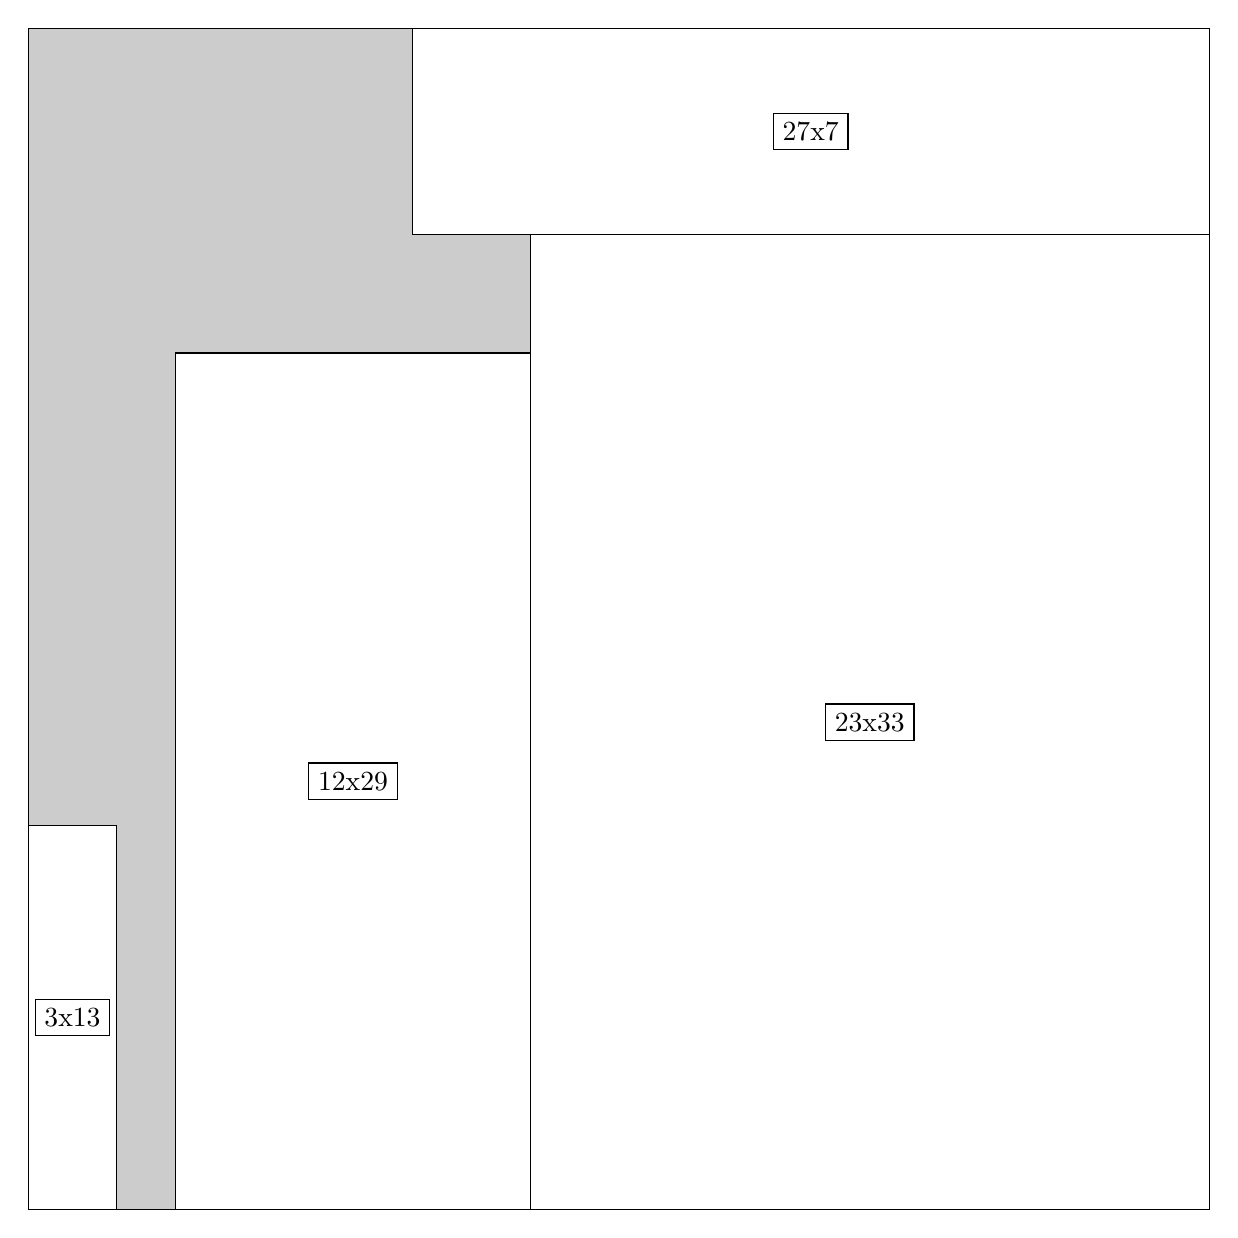
\begin{tikzpicture}[shorten >=1pt,scale=1.0,every node/.style={scale=1.0},->]
\tikzstyle{vertex}=[circle,fill=black!25,minimum size=14pt,inner sep=0pt]
\filldraw[fill=gray!40!white, draw=black] (0,0) rectangle (15.0,15.0);
\foreach \name/\x/\y/\w/\h in {23x33/6.375/0.0/8.625/12.375,12x29/1.875/0.0/4.5/10.875,27x7/4.875/12.375/10.125/2.625,3x13/0.0/0.0/1.125/4.875}
\filldraw[fill=white!40!white, draw=black] (\x,\y) rectangle node[draw] (\name) {\name} ++(\w,\h);
\end{tikzpicture}


w =23 , h =33 , x =17 , y =0 , v =759
\par
w =12 , h =29 , x =5 , y =0 , v =348
\par
w =27 , h =7 , x =13 , y =33 , v =189
\par
w =3 , h =13 , x =0 , y =0 , v =39
\par
\newpage


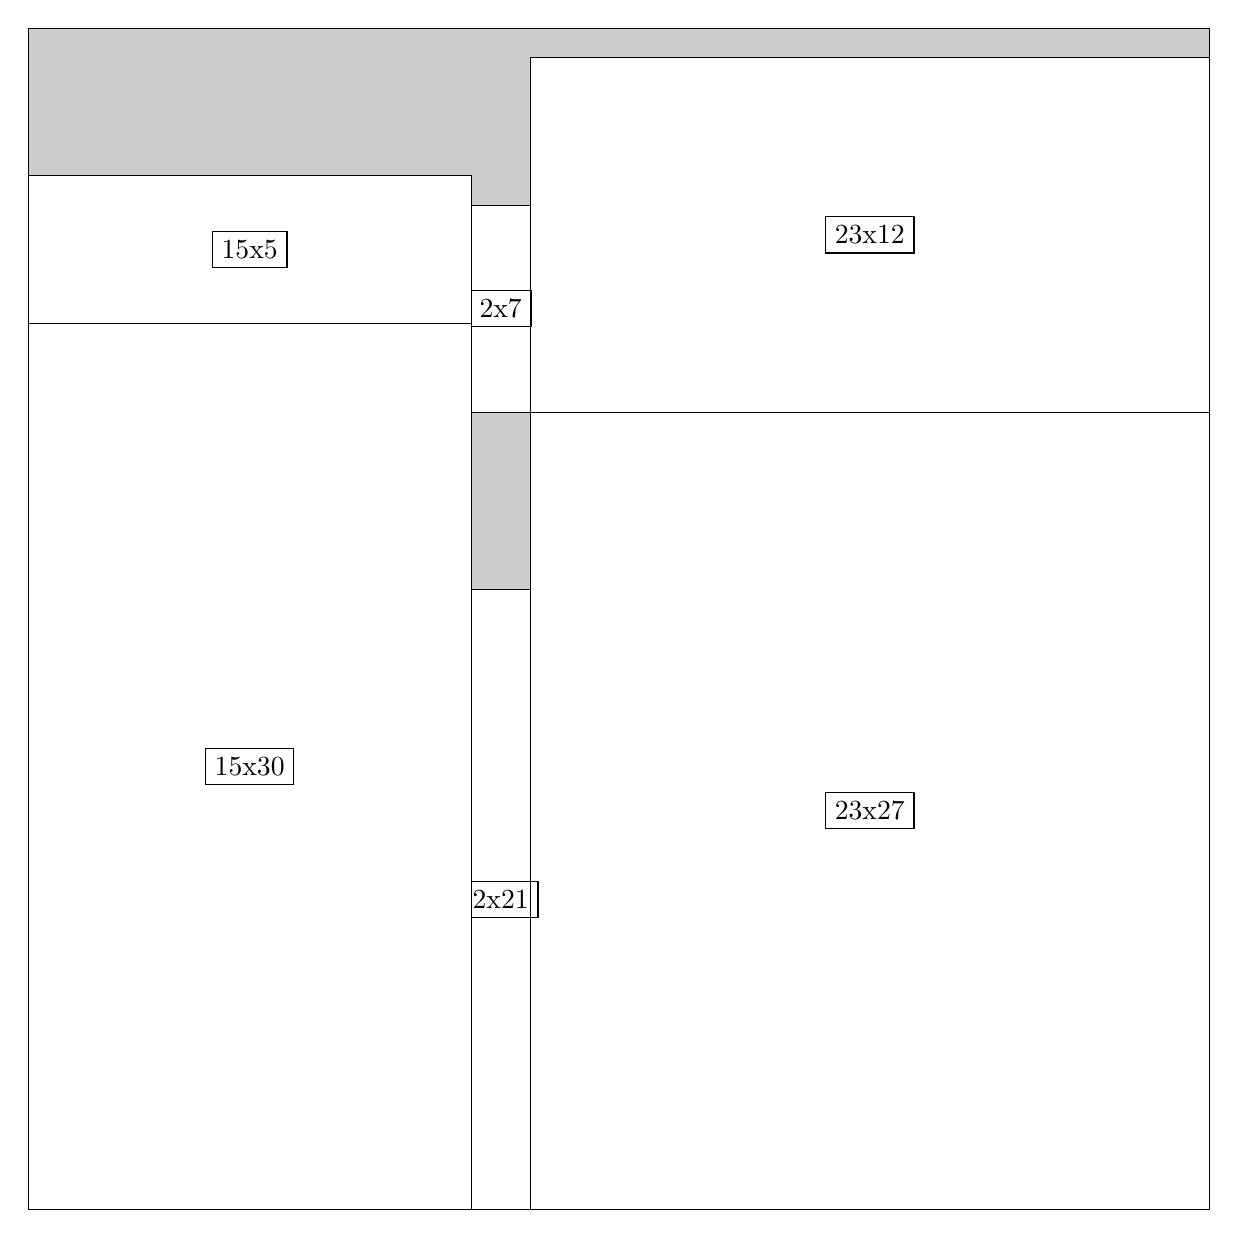
\begin{tikzpicture}[shorten >=1pt,scale=1.0,every node/.style={scale=1.0},->]
\tikzstyle{vertex}=[circle,fill=black!25,minimum size=14pt,inner sep=0pt]
\filldraw[fill=gray!40!white, draw=black] (0,0) rectangle (15.0,15.0);
\foreach \name/\x/\y/\w/\h in {23x27/6.375/0.0/8.625/10.125,2x21/5.625/0.0/0.75/7.875,23x12/6.375/10.125/8.625/4.5,2x7/5.625/10.125/0.75/2.625,15x30/0.0/0.0/5.625/11.25,15x5/0.0/11.25/5.625/1.875}
\filldraw[fill=white!40!white, draw=black] (\x,\y) rectangle node[draw] (\name) {\name} ++(\w,\h);
\end{tikzpicture}


w =23 , h =27 , x =17 , y =0 , v =621
\par
w =2 , h =21 , x =15 , y =0 , v =42
\par
w =23 , h =12 , x =17 , y =27 , v =276
\par
w =2 , h =7 , x =15 , y =27 , v =14
\par
w =15 , h =30 , x =0 , y =0 , v =450
\par
w =15 , h =5 , x =0 , y =30 , v =75
\par
\newpage


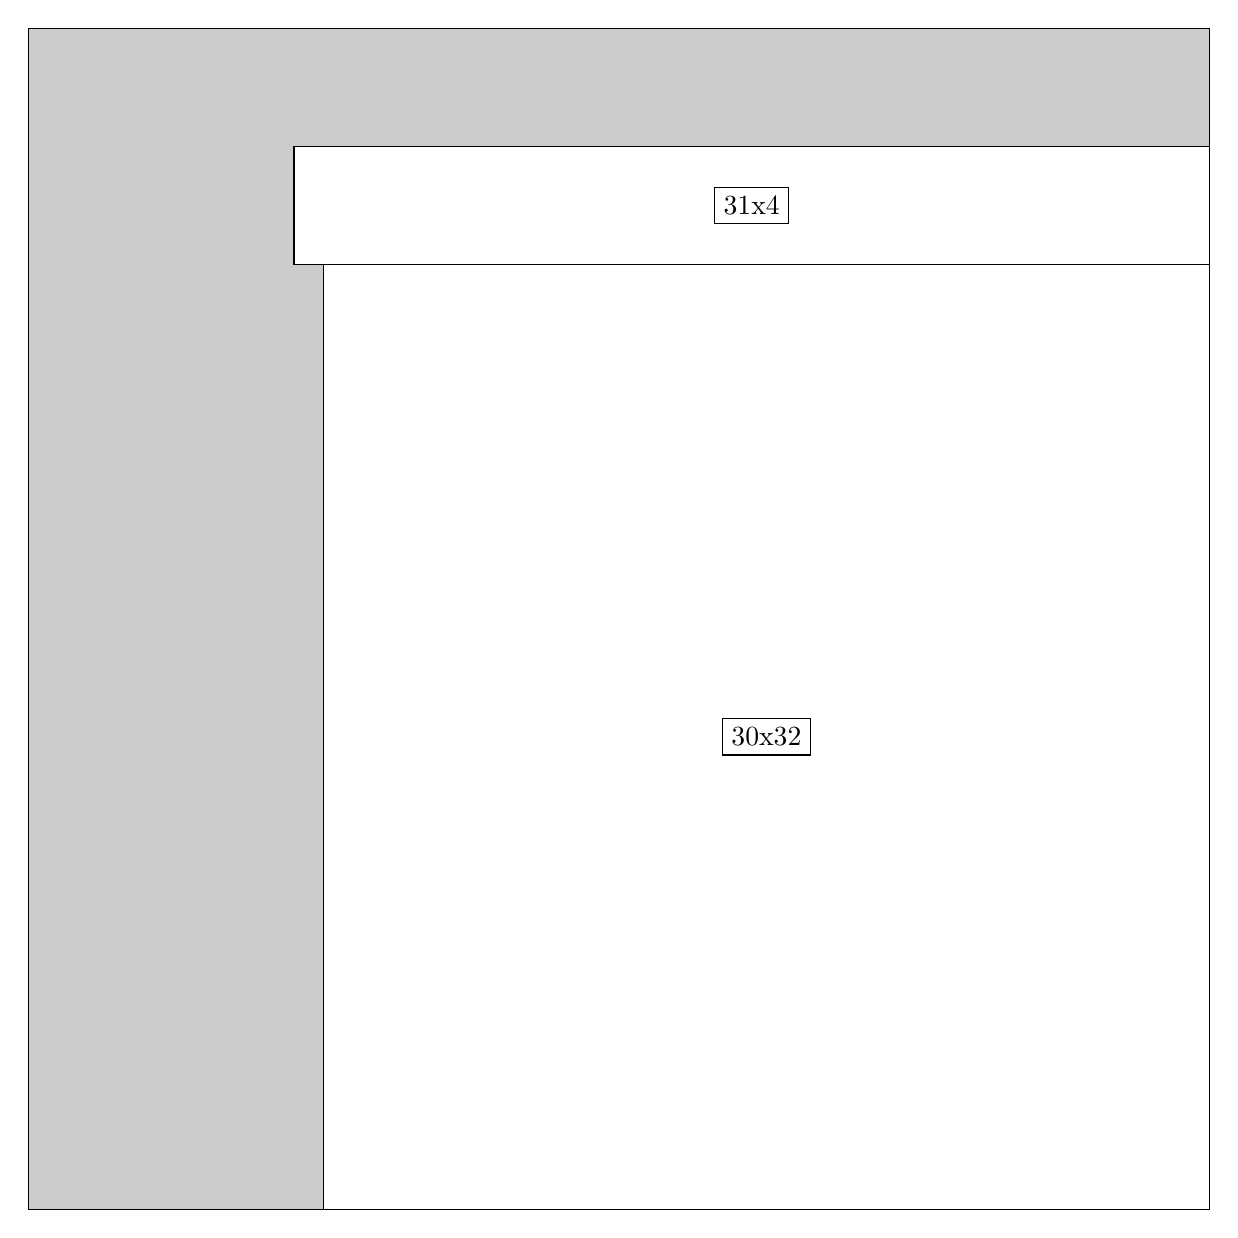
\begin{tikzpicture}[shorten >=1pt,scale=1.0,every node/.style={scale=1.0},->]
\tikzstyle{vertex}=[circle,fill=black!25,minimum size=14pt,inner sep=0pt]
\filldraw[fill=gray!40!white, draw=black] (0,0) rectangle (15.0,15.0);
\foreach \name/\x/\y/\w/\h in {30x32/3.75/0.0/11.25/12.0,31x4/3.375/12.0/11.625/1.5}
\filldraw[fill=white!40!white, draw=black] (\x,\y) rectangle node[draw] (\name) {\name} ++(\w,\h);
\end{tikzpicture}


w =30 , h =32 , x =10 , y =0 , v =960
\par
w =31 , h =4 , x =9 , y =32 , v =124
\par
\newpage


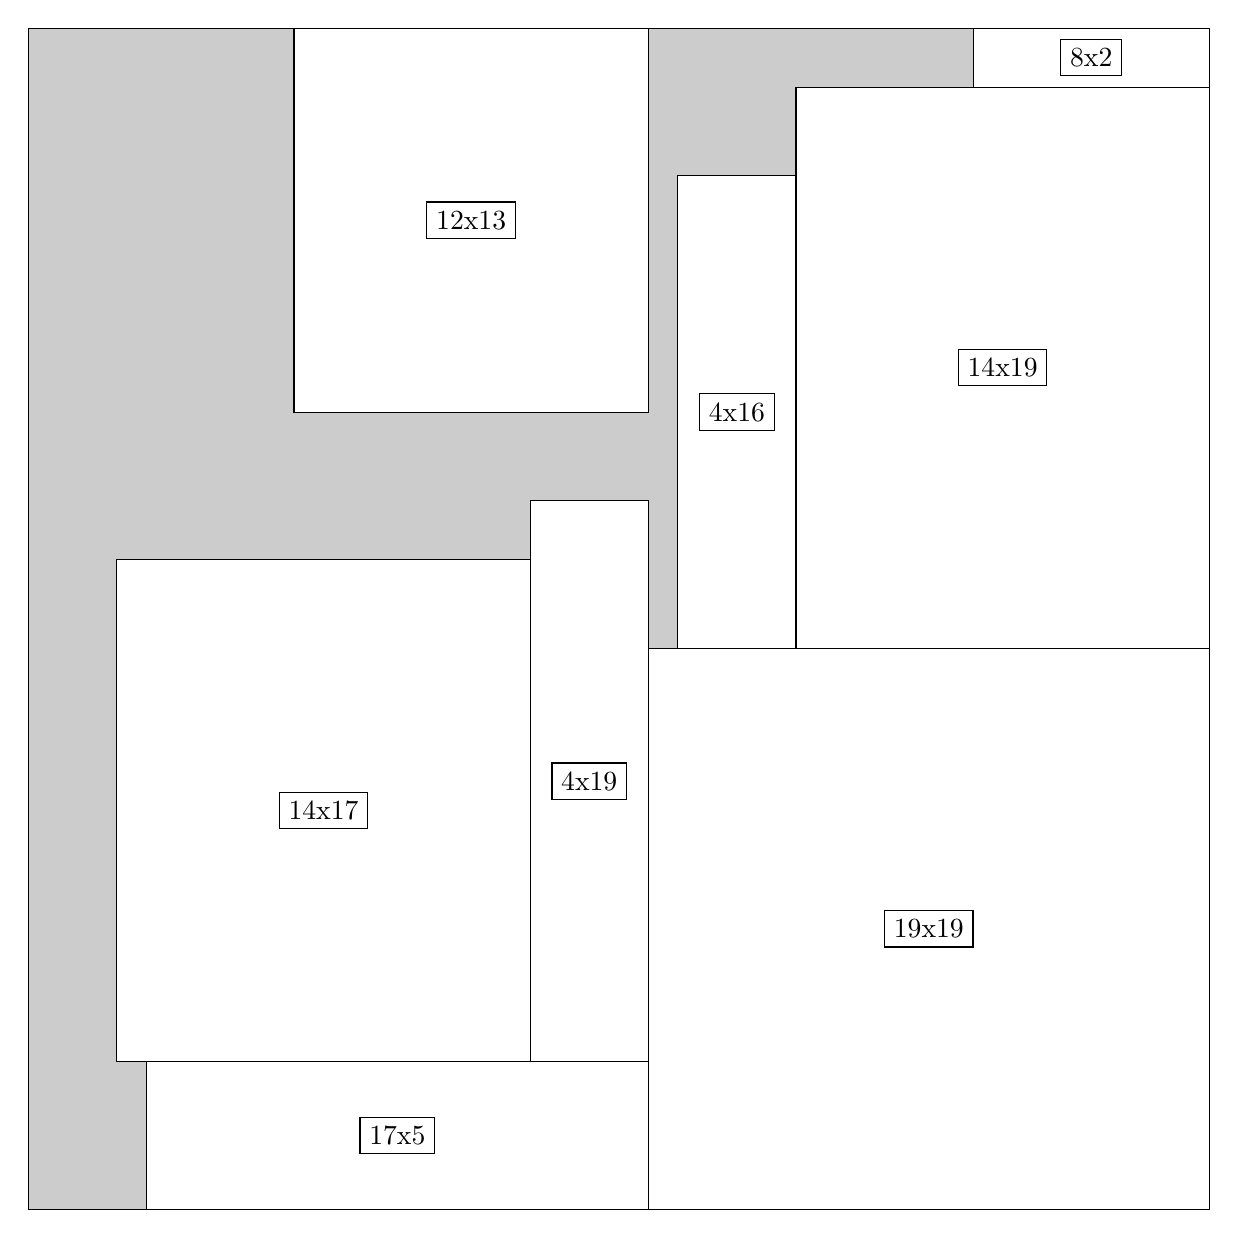
\begin{tikzpicture}[shorten >=1pt,scale=1.0,every node/.style={scale=1.0},->]
\tikzstyle{vertex}=[circle,fill=black!25,minimum size=14pt,inner sep=0pt]
\filldraw[fill=gray!40!white, draw=black] (0,0) rectangle (15.0,15.0);
\foreach \name/\x/\y/\w/\h in {19x19/7.875/0.0/7.125/7.125,14x19/9.75/7.125/5.25/7.125,8x2/12.0/14.25/3.0/0.75,4x16/8.25/7.125/1.5/6.0,17x5/1.5/0.0/6.375/1.875,4x19/6.375/1.875/1.5/7.125,14x17/1.125/1.875/5.25/6.375,12x13/3.375/10.125/4.5/4.875}
\filldraw[fill=white!40!white, draw=black] (\x,\y) rectangle node[draw] (\name) {\name} ++(\w,\h);
\end{tikzpicture}


w =19 , h =19 , x =21 , y =0 , v =361
\par
w =14 , h =19 , x =26 , y =19 , v =266
\par
w =8 , h =2 , x =32 , y =38 , v =16
\par
w =4 , h =16 , x =22 , y =19 , v =64
\par
w =17 , h =5 , x =4 , y =0 , v =85
\par
w =4 , h =19 , x =17 , y =5 , v =76
\par
w =14 , h =17 , x =3 , y =5 , v =238
\par
w =12 , h =13 , x =9 , y =27 , v =156
\par
\newpage


\end{document}